% Created by tikzDevice version 0.12.6 on 2024-08-01 12:50:08
% !TEX encoding = UTF-8 Unicode
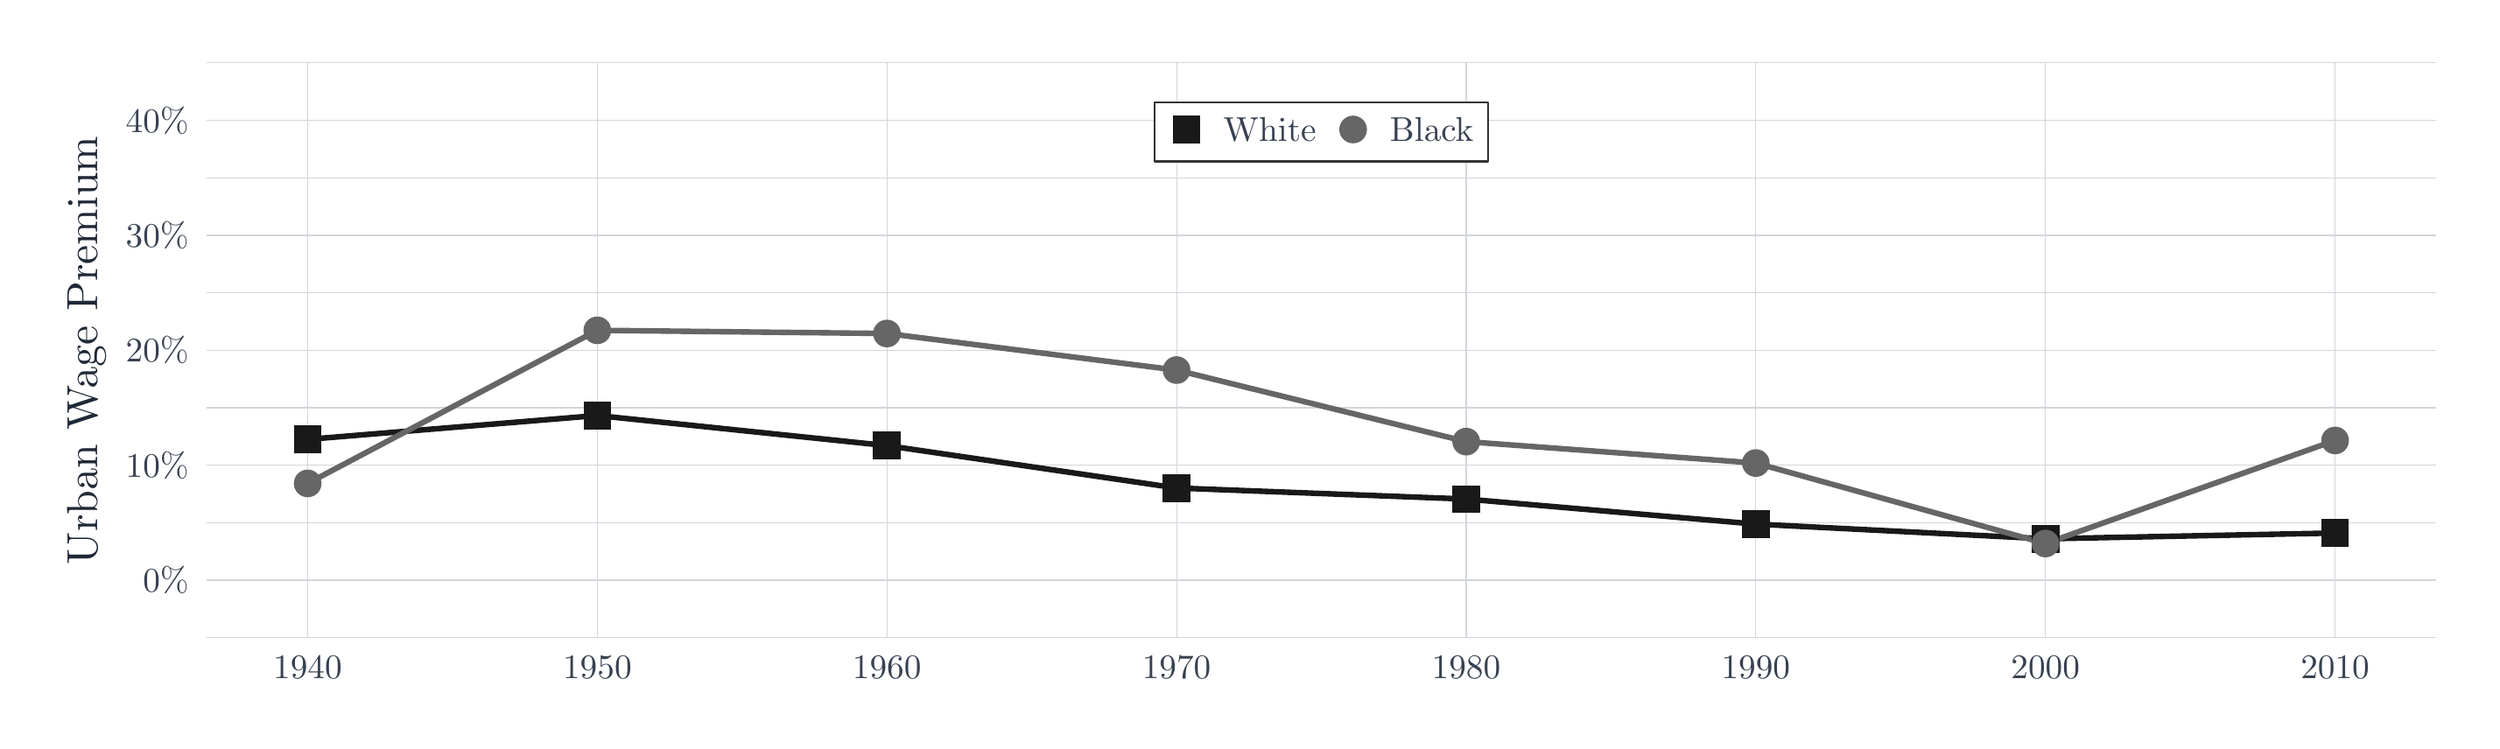
\begin{tikzpicture}[x=1pt,y=1pt]
\definecolor{fillColor}{RGB}{255,255,255}
\path[use as bounding box,fill=fillColor] (0,0) rectangle (1011.78,289.08);
\begin{scope}
\path[clip] (  0.00,  0.00) rectangle (1011.78,289.08);
\definecolor{drawColor}{RGB}{255,255,255}

\path[draw=drawColor,line width= 0.8pt,line join=round,line cap=round,fill=fillColor] (  0.00,  0.00) rectangle (1011.78,289.08);
\end{scope}
\begin{scope}
\path[clip] ( 75.16, 35.76) rectangle (995.78,273.08);
\definecolor{drawColor}{RGB}{255,255,255}
\definecolor{fillColor}{RGB}{255,255,255}

\path[draw=drawColor,line width= 0.8pt,line join=round,line cap=round,fill=fillColor] ( 75.16, 35.76) rectangle (995.78,273.08);
\definecolor{drawColor}{RGB}{209,213,219}

\path[draw=drawColor,line width= 0.4pt,line join=round] ( 75.16, 35.76) --
	(995.78, 35.76);

\path[draw=drawColor,line width= 0.4pt,line join=round] ( 75.16, 83.22) --
	(995.78, 83.22);

\path[draw=drawColor,line width= 0.4pt,line join=round] ( 75.16,130.69) --
	(995.78,130.69);

\path[draw=drawColor,line width= 0.4pt,line join=round] ( 75.16,178.15) --
	(995.78,178.15);

\path[draw=drawColor,line width= 0.4pt,line join=round] ( 75.16,225.62) --
	(995.78,225.62);

\path[draw=drawColor,line width= 0.4pt,line join=round] ( 75.16,273.08) --
	(995.78,273.08);

\path[draw=drawColor,line width= 0.4pt,line join=round] ( 75.16, 59.49) --
	(995.78, 59.49);

\path[draw=drawColor,line width= 0.4pt,line join=round] ( 75.16,106.95) --
	(995.78,106.95);

\path[draw=drawColor,line width= 0.4pt,line join=round] ( 75.16,154.42) --
	(995.78,154.42);

\path[draw=drawColor,line width= 0.4pt,line join=round] ( 75.16,201.88) --
	(995.78,201.88);

\path[draw=drawColor,line width= 0.4pt,line join=round] ( 75.16,249.35) --
	(995.78,249.35);

\path[draw=drawColor,line width= 0.4pt,line join=round] (117.01, 35.76) --
	(117.01,273.08);

\path[draw=drawColor,line width= 0.4pt,line join=round] (236.57, 35.76) --
	(236.57,273.08);

\path[draw=drawColor,line width= 0.4pt,line join=round] (356.13, 35.76) --
	(356.13,273.08);

\path[draw=drawColor,line width= 0.4pt,line join=round] (475.69, 35.76) --
	(475.69,273.08);

\path[draw=drawColor,line width= 0.4pt,line join=round] (595.25, 35.76) --
	(595.25,273.08);

\path[draw=drawColor,line width= 0.4pt,line join=round] (714.81, 35.76) --
	(714.81,273.08);

\path[draw=drawColor,line width= 0.4pt,line join=round] (834.37, 35.76) --
	(834.37,273.08);

\path[draw=drawColor,line width= 0.4pt,line join=round] (953.93, 35.76) --
	(953.93,273.08);
\definecolor{drawColor}{gray}{0.10}

\path[draw=drawColor,line width= 2.3pt,line join=round] (117.01,117.64) --
	(236.57,127.48) --
	(356.13,115.05) --
	(475.69, 97.55) --
	(595.25, 92.98) --
	(714.81, 82.64) --
	(834.37, 76.57) --
	(953.93, 78.95);
\definecolor{drawColor}{gray}{0.40}

\path[draw=drawColor,line width= 2.3pt,line join=round] (117.01, 99.44) --
	(236.57,162.66) --
	(356.13,161.35) --
	(475.69,146.25) --
	(595.25,116.70) --
	(714.81,107.85) --
	(834.37, 74.62) --
	(953.93,117.18);
\definecolor{fillColor}{gray}{0.10}

\path[fill=fillColor] (111.30,111.93) --
	(122.72,111.93) --
	(122.72,123.35) --
	(111.30,123.35) --
	cycle;
\definecolor{fillColor}{gray}{0.40}

\path[fill=fillColor] (117.01, 99.44) circle (  5.71);
\definecolor{fillColor}{gray}{0.10}

\path[fill=fillColor] (230.86,121.77) --
	(242.28,121.77) --
	(242.28,133.19) --
	(230.86,133.19) --
	cycle;
\definecolor{fillColor}{gray}{0.40}

\path[fill=fillColor] (236.57,162.66) circle (  5.71);
\definecolor{fillColor}{gray}{0.10}

\path[fill=fillColor] (350.42,109.34) --
	(361.84,109.34) --
	(361.84,120.76) --
	(350.42,120.76) --
	cycle;
\definecolor{fillColor}{gray}{0.40}

\path[fill=fillColor] (356.13,161.35) circle (  5.71);
\definecolor{fillColor}{gray}{0.10}

\path[fill=fillColor] (469.98, 91.84) --
	(481.40, 91.84) --
	(481.40,103.26) --
	(469.98,103.26) --
	cycle;
\definecolor{fillColor}{gray}{0.40}

\path[fill=fillColor] (475.69,146.25) circle (  5.71);
\definecolor{fillColor}{gray}{0.10}

\path[fill=fillColor] (589.54, 87.27) --
	(600.96, 87.27) --
	(600.96, 98.69) --
	(589.54, 98.69) --
	cycle;
\definecolor{fillColor}{gray}{0.40}

\path[fill=fillColor] (595.25,116.70) circle (  5.71);
\definecolor{fillColor}{gray}{0.10}

\path[fill=fillColor] (709.10, 76.93) --
	(720.52, 76.93) --
	(720.52, 88.35) --
	(709.10, 88.35) --
	cycle;
\definecolor{fillColor}{gray}{0.40}

\path[fill=fillColor] (714.81,107.85) circle (  5.71);
\definecolor{fillColor}{gray}{0.10}

\path[fill=fillColor] (828.66, 70.86) --
	(840.08, 70.86) --
	(840.08, 82.28) --
	(828.66, 82.28) --
	cycle;
\definecolor{fillColor}{gray}{0.40}

\path[fill=fillColor] (834.37, 74.62) circle (  5.71);
\definecolor{fillColor}{gray}{0.10}

\path[fill=fillColor] (948.22, 73.24) --
	(959.64, 73.24) --
	(959.64, 84.66) --
	(948.22, 84.66) --
	cycle;
\definecolor{fillColor}{gray}{0.40}

\path[fill=fillColor] (953.93,117.18) circle (  5.71);
\end{scope}
\begin{scope}
\path[clip] (  0.00,  0.00) rectangle (1011.78,289.08);
\definecolor{drawColor}{RGB}{55,65,81}

\node[text=drawColor,anchor=base east,inner sep=0pt, outer sep=0pt, scale=  1.42] at ( 67.96, 54.59) {0\%};

\node[text=drawColor,anchor=base east,inner sep=0pt, outer sep=0pt, scale=  1.42] at ( 67.96,102.06) {10\%};

\node[text=drawColor,anchor=base east,inner sep=0pt, outer sep=0pt, scale=  1.42] at ( 67.96,149.52) {20\%};

\node[text=drawColor,anchor=base east,inner sep=0pt, outer sep=0pt, scale=  1.42] at ( 67.96,196.99) {30\%};

\node[text=drawColor,anchor=base east,inner sep=0pt, outer sep=0pt, scale=  1.42] at ( 67.96,244.45) {40\%};
\end{scope}
\begin{scope}
\path[clip] (  0.00,  0.00) rectangle (1011.78,289.08);
\definecolor{drawColor}{RGB}{55,65,81}

\node[text=drawColor,anchor=base,inner sep=0pt, outer sep=0pt, scale=  1.42] at (117.01, 18.76) {1940};

\node[text=drawColor,anchor=base,inner sep=0pt, outer sep=0pt, scale=  1.42] at (236.57, 18.76) {1950};

\node[text=drawColor,anchor=base,inner sep=0pt, outer sep=0pt, scale=  1.42] at (356.13, 18.76) {1960};

\node[text=drawColor,anchor=base,inner sep=0pt, outer sep=0pt, scale=  1.42] at (475.69, 18.76) {1970};

\node[text=drawColor,anchor=base,inner sep=0pt, outer sep=0pt, scale=  1.42] at (595.25, 18.76) {1980};

\node[text=drawColor,anchor=base,inner sep=0pt, outer sep=0pt, scale=  1.42] at (714.81, 18.76) {1990};

\node[text=drawColor,anchor=base,inner sep=0pt, outer sep=0pt, scale=  1.42] at (834.37, 18.76) {2000};

\node[text=drawColor,anchor=base,inner sep=0pt, outer sep=0pt, scale=  1.42] at (953.93, 18.76) {2010};
\end{scope}
\begin{scope}
\path[clip] (  0.00,  0.00) rectangle (1011.78,289.08);
\definecolor{drawColor}{RGB}{31,41,55}

\node[text=drawColor,rotate= 90.00,anchor=base,inner sep=0pt, outer sep=0pt, scale=  1.80] at ( 30.15,154.42) {Urban Wage Premium};
\end{scope}
\begin{scope}
\path[clip] (  0.00,  0.00) rectangle (1011.78,289.08);
\definecolor{drawColor}{gray}{0.20}
\definecolor{fillColor}{RGB}{255,255,255}

\path[draw=drawColor,line width= 0.8pt,line join=round,line cap=round,fill=fillColor] (466.59,232.37) rectangle (604.35,256.83);
\end{scope}
\begin{scope}
\path[clip] (  0.00,  0.00) rectangle (1011.78,289.08);
\definecolor{drawColor}{RGB}{255,255,255}
\definecolor{fillColor}{RGB}{255,255,255}

\path[draw=drawColor,line width= 0.8pt,line join=round,line cap=round,fill=fillColor] (472.59,238.37) rectangle (487.04,252.83);
\end{scope}
\begin{scope}
\path[clip] (  0.00,  0.00) rectangle (1011.78,289.08);
\definecolor{fillColor}{gray}{0.10}

\path[fill=fillColor] (474.10,239.89) --
	(485.52,239.89) --
	(485.52,251.31) --
	(474.10,251.31) --
	cycle;
\end{scope}
\begin{scope}
\path[clip] (  0.00,  0.00) rectangle (1011.78,289.08);
\definecolor{drawColor}{RGB}{255,255,255}
\definecolor{fillColor}{RGB}{255,255,255}

\path[draw=drawColor,line width= 0.8pt,line join=round,line cap=round,fill=fillColor] (541.35,238.37) rectangle (555.80,252.83);
\end{scope}
\begin{scope}
\path[clip] (  0.00,  0.00) rectangle (1011.78,289.08);
\definecolor{fillColor}{gray}{0.40}

\path[fill=fillColor] (548.57,245.60) circle (  5.71);
\end{scope}
\begin{scope}
\path[clip] (  0.00,  0.00) rectangle (1011.78,289.08);
\definecolor{drawColor}{RGB}{55,65,81}

\node[text=drawColor,anchor=base west,inner sep=0pt, outer sep=0pt, scale=  1.42] at (495.04,240.70) {White};
\end{scope}
\begin{scope}
\path[clip] (  0.00,  0.00) rectangle (1011.78,289.08);
\definecolor{drawColor}{RGB}{55,65,81}

\node[text=drawColor,anchor=base west,inner sep=0pt, outer sep=0pt, scale=  1.42] at (563.80,240.70) {Black};
\end{scope}
\end{tikzpicture}
